\documentclass[11pt,a4paper]{jsarticle}

\usepackage[dvipdfmx]{graphicx}
\setlength{\textwidth}{\fullwidth}
\setlength{\textheight}{39\baselineskip}
\addtolength{\textheight}{\topskip}
\setlength{\voffset}{-0.2in}
\setlength{\topmargin}{0pt}
\setlength{\headheight}{0pt}
\setlength{\headsep}{0in}

\title{\Huge{プロジェクトマネジメント演習1\\第2班 報告書}}
\author{158576C 新里亮太}
\date{\today}

\begin{document}
\maketitle\thispagestyle{empty}
\newpage
\tableofcontents\thispagestyle{empty}
\newpage

\pagenumbering{arabic}
\setcounter{page}{1}




\section{プロジェクト憲章}
\subsection{プロジェクト名と概要}


本プロジェクトは、「ホログラムで広がる無限の世界」と題し、現在研究・開発が進んでいるホログラム技術と、Fairy Lightsという技術を組み合わせて部屋に投影することで部屋の内装などを変更する。
\subsection{メンバーと組織}
学部生
\begin{itemize}
\item 155702F 大城由也
\item 155708E 中村孝道
\item 155743C 平良柚那
\item 155750F 翁長泰司
\item 155756E 金城愛梨
\item 155757C 平本嶺河
\end{itemize}

院生
\begin{itemize}
\item 158574G 比嘉健太
\item 158576C 新里亮太  
\end{itemize}


\subsection{目標}
部屋の模様替えをする際、かなりのコストと労働力が必要となる。また、宇宙空間や大自然の中で生活することは現代社会に生きる私たちにとって非現実的であると言える。更に、、アレルギーや危険性などで部屋で飼うことのできない動物などもある。これらの問題を解決するために、触ることのできるホログラム技術を用いて部屋の内装を変更したり、動物を投影する。

\subsection{独自性と制約}
独自性
\begin{itemize}
\item プロジェクトメンバーの全員が情報工学科の学生である
\item 触れるホログラムを用いて部屋の内装などを変更する
\item ホログラム投影機を一般家庭に普及させる
\item 現段階では研究中の技術であるFariy Lightsを用いて企画を行う
\end{itemize}

制約
\begin{itemize}
\item 資金がない
\item 講義やアルバイトなどで全員が同じ時間仕事できるわけではない
\item 院生を含めたミーティングが週に一度しかない
\item プレゼンテーションに慣れているメンバーが居ない
\end{itemize}

\subsection{成果物}
\begin{itemize}
\item 発表用スライド
\item 最終報告書
\item 予稿
\end{itemize}

\subsection{日程と終了}
\subsubsection{日程}
\begin{itemize}
\item 6月12日 第一回ミーティング
\begin{itemize}
\item ブレーンストーミングによるアイディア出し
\item 成果物報告場所の作成(GoogleDriveにて共有)
\end{itemize}
\item 6月16日 第二回ミーティング
\begin{itemize}
\item テーマ決定
\item ホログラムを用いて何ができるのか話し合い
\end{itemize}
\item 7月3日 第三回ミーティング
\begin{itemize}
\item 中間発表練習
\end{itemize}
\item 7月5日 第四回ミーティング
\begin{itemize}
\item 中間発表練習
\end{itemize}
\item 7月6日 中間発表
\item 7月17日 第五回ミーティング
\begin{itemize}
\item 最終発表の仮原稿添削
\end{itemize}
\item 7月24日 第六回ミーティング
\begin{itemize}
\item 最終報告書添削
\end{itemize}
\item 8月6日 第七回ミーティング
\begin{itemize}
\item 最終発表スライド添削
\end{itemize}
\item 8月7日 第八回ミーティング
\begin{itemize}
\item 最終発表原稿添削
\end{itemize}
\item 8月12日 第九回ミーティング
\begin{itemize}
\item 第一回発表練習
\end{itemize}
\item 8月13日 第十回ミーティング
\begin{itemize}
\item 第二回発表練習
\end{itemize}
\item 8月14日 最終発表
\end{itemize}

\subsubsection{終了}
\begin{itemize}
\item 8月14日のPD最終発表にて発表する。また、スライドや予稿の提出も期限内に行う。
\end{itemize}


\section{プロジェクト計画・実績}
\subsection{目標とスコープ}
\subsubsection{目標}
8月14日のプロジェクトデザイン最終発表にて発表する。また、スライド、予稿を期限内に提出する。
\subsubsection{スコープ}
以下にプロダクトスコープを示す
\begin{itemize}
\item 最終発表スライド
\begin{itemize}
\item 8月14日までにアップロードする
\item 12分の発表に十分収まるスライドを作成する
\end{itemize}
\item 最終報告書
\begin{itemize}
\item 6ページの最終報告書を作成する
\item 企画内容や新規性・社会性など指定された内容を記述する
\end{itemize}
\item 予稿
\begin{itemize}
\item 企画内容やメンバーなどを指定の場所にアップロードする
\item 発表スライドをアップロードする
\end{itemize}
\end{itemize}

\subsection{WBSとアクティビティ}
以下にWBSを示す。
\newpage

\begin{figure}[htbp]
\begin{center}
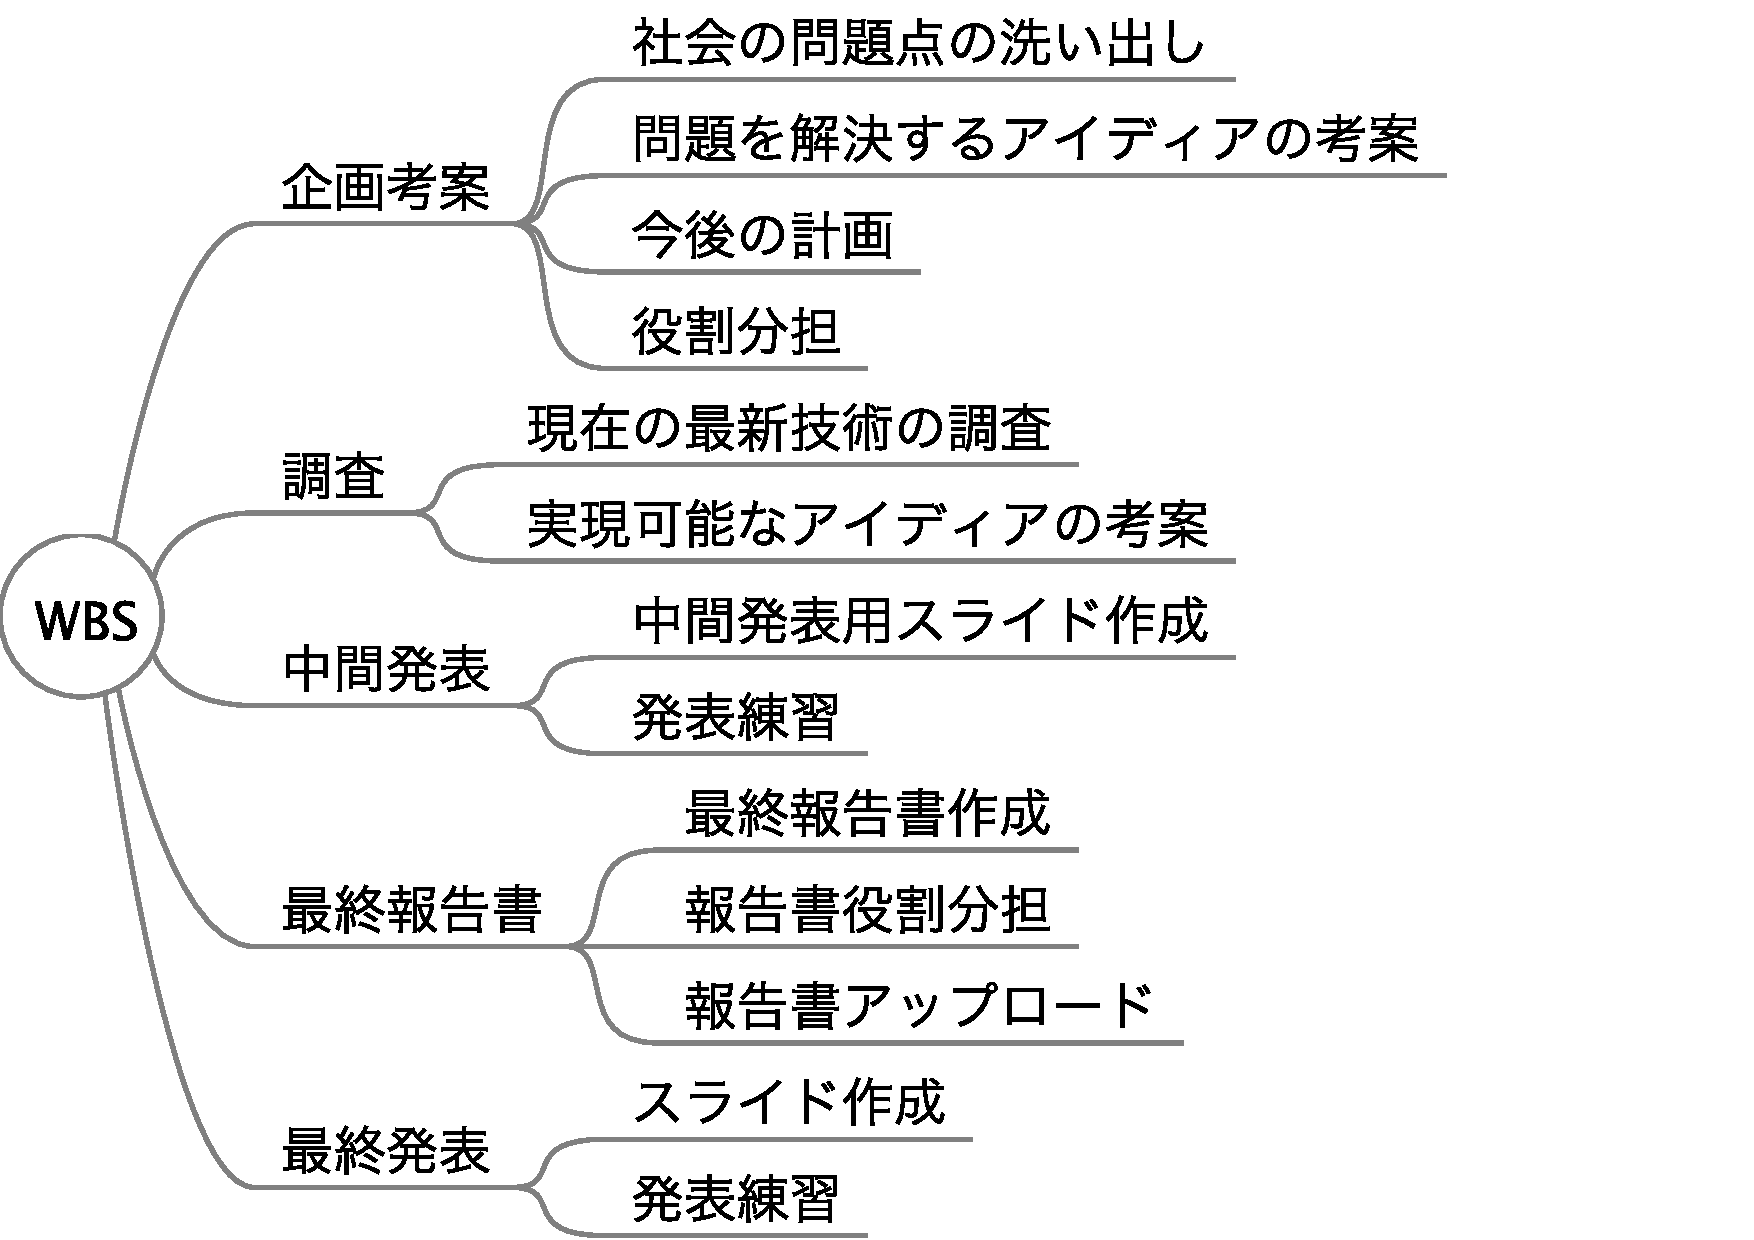
\includegraphics[width=10cm]{wbs.pdf}
\end{center}
\caption{WBS}
\end{figure}

\subsection{スケジュール}
以下にガントチャートを示す。赤が予定していたスケジュールで、青が実際のスケジュールである

\begin{figure}[htbp]
\begin{center}
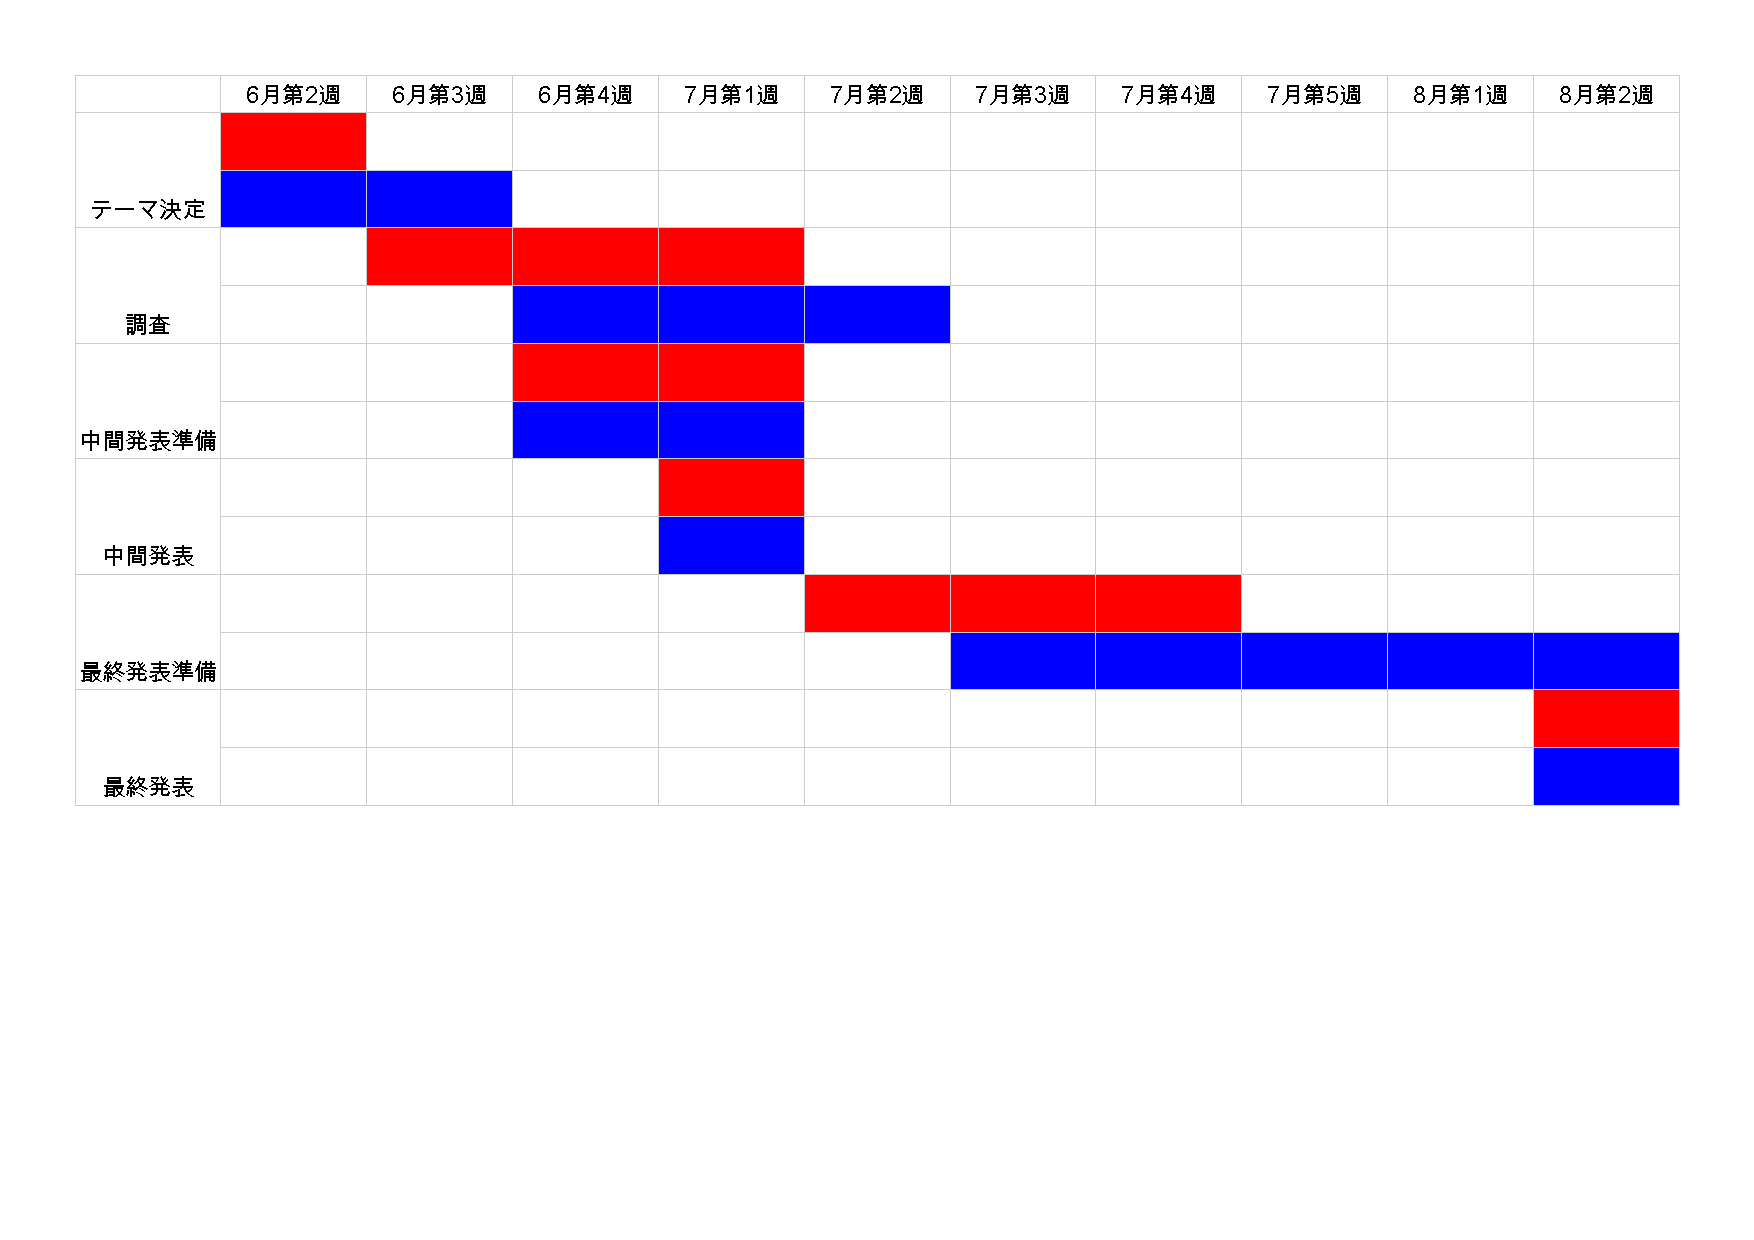
\includegraphics[width=10cm]{gant.pdf}
\end{center}
\caption{ガントチャート}
\end{figure}

\subsection{リスクと課題}
予見されるリスクとその解決策を以下に示す。

\begin{itemize}
\item 来なくなるメンバーが出る\\
実際に集まりへの参加率が低いメンバーはいたが、こまめに連絡を取ることで全く来ないメンバーは出なかった。
\item メンバーと連絡が取れなくなる\\
メンバーと連絡が取れなくなることはなかったが、参加率が低いメンバーには直接声をかけるなどした。
\item 仕事をしないメンバーが出る\\
メンバーそれぞれに仕事を分担し、仕事が難しいメンバーにはサポートを付けて仕事に取り組ませた。
\item 成果物が最終発表に間に合わない\\
最終発表に間に合わせるため、毎回のミーティングでスケジュールを確認し遅れている場合はミーティングを増やすなどした。
\end{itemize}

\subsection{チームとコミュニケーション}
利用したコミュニケーションツールを以下に示す。

\begin{itemize}
\item LINE\\
日々の連絡はLINEを用いた。LINEには既読マークがあり、最低限目を通したかどうかは確認できるためある程度有効だった。
\item GoogleDrive\\
議事録や成果物の管理はGoogleDriveを用いた。また、次回のミーティングの連絡はGoogleDriveにアップロードされる議事録とLINEを用いて二重に連絡した。
\end{itemize}

\subsection{実績と品質}
成果物の評価は2名のPMで行った。具体的にチェックした項目を以下に示す。

\begin{itemize}
\item 新規性・社会性・有効性はあるか
\item 企画内容は実現可能か
\item 十分に調査がなされているか
\item 最終報告書・発表スライドは論理的な展開になっているか
\end{itemize}


\subsection{応用}
今回は2名のPMが付いたが、メインPMとサブPMで分けて、班活動の指揮はメインPMが執る。どちらのPMも互いに意見を出しあいより良い企画になるようアドバイスを送った。
基本的に互いのPMの意思が統一されていたので方針はメインPMに任せていた。


\section{終結}
\subsection{概要}
プロジェクト開始後、まずはリーダーと議事録係を決めた。その後、ブレーンストーミングを行いテーマを決定した。ブレーンストーミングに慣れていないメンバーが多いようだったので、PMが適宜アドバイスや問いかけをしながら議論が円滑に進むようにした。その後は週に一回のPMも交えたミーティングと適宜メンバーだけのミーティングを行った。

ミーティングでは毎回議事録や資料を作成させ、GoogleDriveにアップロードさせることで後からメンバーが見返せるようにした。

中間発表・最終発表前には発表練習を行い、より良い発表になるようPMからアドバイスをし、適宜スライドの添削などを行った。スライドにはまとめページや質問回答用ページを用意させるなどより伝わりやすい発表を目指した。また、PD2と一緒に発表練習を行うことで先輩の発表を見せ、良い刺激を与えたのではないかと思う。

最終報告書はまず草案を作成させ、2名のPMでかなり細かいところまで指摘し添削した。また、最終報告書草案の作成時点で最終発表を想定しながら作成させた。

最終発表二日前と前日で発表練習をし、最終発表を迎えた。二回の発表練習を行っているだけあって、PMとしてはある程度満足できる発表になった。最終発表をもってプロジェクトを終了とした。

\subsection{メンバー評価}
ルーブリック法にて各メンバーとPMを評価した。評価はAからFまでの5段階評価になっており、それぞれの評価を統合したものを以下に示す。


\begin{itemize}
\item 155702F 大城由也 B\\
最終報告書草案作成など、与えられた仕事をきちんとこなした。また、企画のキャッチフレーズを考案するなど文章作成の仕事で能力を発揮していた。仕事をしっかりこなすのでメンバーからの評価も高かった。ミーティングでは少し発言が少なかったとの意見も出ていた。

\item 155708E 中村考道 D\\
最終報告書草案作成など、与えられた仕事はしていたようだった。ミーティングへの参加率の低さや、参加してもあまり話を聞いてないことなどからメンバーからの評価は低かったが、鋭い意見を出すなどで多少の評価を得ていた。

\item 155743C 平良柚那 A\\
リーダーとして班をまとめた。自ら率先して仕事を行った。また、他のメンバーの仕事も積極的にサポートし、メンバーからの信頼を得ていた。PMにアドバイスを求めに来るときも彼女の方から積極的に動き、常にどうしたらよりよい企画になるか考えていた。

\item 155750F 翁長泰司 C\\
主にスライド作成係として活動した。ブレーンストーミングの際に積極的に発言するなどして議論を盛り上げた。与えられた仕事を自主的にできていなかったが、PMからの指摘を真摯に受け止めスライドを完成させた。自分の仕事が終わるとミーティングでの積極性が少し失われた。

\item 155756E 金城愛梨 A\\
議事録係として毎回のミーティングの議事録・マインドマップ作成を行った。また、議論の際に積極的に意見やアイディアを出し議論を盛り上げた。発表係としても活動し、原稿作成や当日の発表など大きな仕事をこなした。リーダーと並んでグループの中心人物だった。

\item 155757C 平本嶺河 C\\
最終報告書作成係として活動した。与えられた仕事はしっかりこなし、わからないところは自分から聞くなどして仕事を完遂しようと努力した。議論の際に積極性に欠け、自分から発言することが少なかったように思えるが、ミーティングへの出席率は高かった。

\item 158574G 比嘉健太 A\\
サブPMとして活動し、議論の際に様々な意見を出すなどしてメンバーからの信頼も厚かった。

\item 158576C 新里亮太 A\\
メインPMとして活動し、グループ活動を指揮した。
\end{itemize}


\subsection{プロジェクト評価}
成果物を期限内に完成させ最終発表を行った点では評価できる。企画内容の掘り下げを行うタイミングが遅れてしまい、内容としては多少不十分だった点もある。

企画が実現できるかどうかの調査はしっかりできており、研究・開発が進んでいる技術を企画に取り入れるなど現実性のある企画ができた。

メンバー間のコミュニケーションは取れており、完全に参加しなくなるメンバーが出なかった点は幸いである。

\subsection{教訓}
企画立案の際には、最初の段階で内容の掘り下げを行う必要があることを知った。最終報告書作成やスライド作成時点で慌てて企画を掘り下げ始めると内容が二転三転して思うようにまとまらなかった。

\subsection{講義}
PDに関してはテーマ設定の見直しが必要であると思われる。テーマが抽象的なため、様々な案が出る可能性はあるが、例年よく見る企画(メガフロート、鉄道、沖縄と本州を結ぶトンネル等)が多くありPM側としてはどう企画を決定するか悩ましい部分もあった。

最終発表を見て、調査の重要性を講義で取り上げる必要があるように感じた。調査が不十分でデータに基づく企画がなされていないようであった。

PM演習の講義に関しては、互いのグループの進捗状況や問題点を共有できて有意義だったと思う。また、他学科の活動についても知ることができ互いに刺激になったと思う。


\end{document}
